In this section, we present general concepts related to cloud database management in order to provide a better understanding of the key issues that affect data consistency. Initially, we approach the architectural aspects of the DBaaS model. After that, we highlight the cloud storage infrastructure requirements and describe the ACID properties. Finally, we introduce the CAP theorem and discuss its associated trade-offs. 
\vspace{1mm}

\subsection{Architectural Aspects of the DBaaS \\ Model}

In the DBaaS model, the architecture is often distributed and data can be stored in possibly hundreds of machines, where the resources are shared among the clients~\cite{Xiong:2011}. As previously mentioned, one of the techniques used to obtain %various 
{\al specific} features
such as fast access, improved performance and high availability is to replicate data in geographically distinct locations.  % Hence, replication is an essential resource in the DBaaS model. % Repetido da introdução

{\al For example, in a scenario in which a failure occurs} in a replica, possibly the system will continue to operate by switching  requests between the replicas. Another benefit is scalability, {\al which allows} the system to handle an increase in the number of requests as well as in the volume of stored data \cite{tanenbaum:2007}. Once considering the possibility of data replication in geographically distant areas, it is necessary to define how updates will be spread among the replicas, since the manner how this operation is {\al executed directly affects data consistency.}
%will be addressed can directly affect data consistency.

Data partitioning represents another distribution method in the DBaaS model. It is performed by breaking a table into two or more fragments or partitions, which can be stored in different locations~\cite{RahimiHaug:2010}. This method differs from replication in the sense that instead of copying the data it splits them according to certain criteria. 
%rather than copying the data, we have the division of them, according to certain criteria. 
In cloud environments, partitioning may occur dynamically and in real time.

\subsection{Cloud Data Storage Requirements}

A trustworthy and appropriate data storage infrastructure is a key aspect to achieve an adequate cloud database management, {\al so that} all resources can be efficiently utilized and shared to reduce consistency issues. Therefore, {\dg the following} 
are some needed and crucial requirements that must be considered in a shared infrastructure model~\cite{ju2011survey, rimal2009taxonomy}.\\

\noindent
\textbf{Automation.} The data storage must be automated to be able to quickly execute infrastructure changes necessary to meet the previous requirements without human intervention.

{\rc 
\noindent
\textbf{Availability.} The data storage must ensure that data continues to be available at a required level of performance in situations ranging from normal to adverse.
}

\noindent
\textbf{Elasticity.} Not only must the data storage be able to scale with increasing load, {\al but} it must also be able to adjust to reductions in load by releasing cloud resources, while guaranteeing compliance with any Service Level Agreement (SLA).
%The data storage must enable a rapid adjustment of {\al its} infrastructure to {\al deal with} the increasing demand and {\dg guarantee} the compliance with any Service Level Agreements (SLAs).

\noindent
\textbf{Fault Tolerance.} The data storage must be able to recover in case of failure by providing a backup instance of the application that will be ready to take over without disruption.

\noindent
\textbf{Low Latency.} The data storage must handle latency issues by measuring and testing the network latency before committing an application.

\noindent
\textbf{Performance.} The data storage must {\al provide} an infrastructure that {\al supports} fast and robust data access, update and recovery.

\noindent
\textbf{Reliability.} The data storage must ensure that the data {\dg can be recovered} in case a disaster {\dg occurs}.

\noindent
\textbf{Scalability.} The data storage needs to quickly scale to meet workload demands, % huge capacities, 
%so that it must provide 
providing horizontal and vertical scalability. Horizontal scalability  refers to the ability to increase capacity by adding more machines or setting up a new cluster or a new distributed environment. Vertical scalability, on the other hand, refers to the increase of capacity by adding more resources %such as more memory or an additional CPU,  
{\al to a machine (\emph{e.g.}, more memory or an additional CPU).}

\subsection{The ACID Properties}

Conventional Database Management Systems must conform to four transaction properties: \textit{Atomicity}, \textit{Consistency}, \textit{Isolation} and \textit{Durability}. Known as the ACID properties, %these properties have already been 
they are well discussed in the literature~\cite{acid1983}, existing several approaches to achieve them. However, in the DBaaS model, due to architectural aspects previously described, assuring the ACID {properties} is a nontrivial task.

Despite the difficulty for assuring the ACID properties in a cloud data storage, strategies have been proposed in the attempt to manage them in web application transactions. For instance, atomicity might be guaranteed by implementing the two-phase commit (2PC) protocol~\cite{gray1978dbos}. Isolation can be obtained by a multi-version concurrency control %(MVCC) 
or by a global timestamp, while durability can be achieved by applying queuing strategies such as FIFO (\emph{First In, First Out}) to concurrent write transactions, so that old updates do not override the latest ones~\cite{Wei:2009}. 

However, replication represents an important obstacle to guarantee consistency~\cite{Abadi09}. %The main\-te\-nance of 
{\al Thus, mantaining a} replicated database in a mutually consistent state implies that in all of its replicas each of their data items must have identical values~\cite{OzsuValduriez:2011}. Therefore, strategies for data update and propagation must be implemented to ensure that, if a copy is updated, all the other ones must be updated too~\cite{tanenbaum:2007}.

\subsection{The CAP Theorem}

%Brewer \cite{Brewer2000} introduced the CAP theorem, which was subsequently proved by Gilbert and  Lynch~\cite{Gilbert:2002}. 
The CAP theorem was introduced by Brewer as a conjecture~\cite{Brewer2000} and subsequently proved 
{\dg (in  a restricted form)} by Gilbert and  Lynch~\cite{Gilbert:2002}. 
{\dg Since then it has become an important concept in cloud systems~\cite{brewer2012}.}
It establishes that, when considering the desirable properties of \textit{Consistency}, \textit{Availability}, and \textit{Partition tolerance} in distributed systems, at most two of them can be achieved simultaneously.

It is evident that %the implications of the CAP theorem introduced conflicts and
the CAP theorem introduces conflicts and imposes several challenges to dis\-trib\-uted systems and service providers. Among the conflicts derived from it, considering that network partitions are inevitable in a geographically distributed scenario, we highlight the trade-off between Consistency and Availability~\cite{gilbert2012perspectives}. To illustrate this situation, in Figure~\ref{fig:figure1} we observe that User~2 performs a read request for data item D1 in replica R3 (Da\-ta\-center~2), after User~1 has updated data item D1 in replica R1 (Datacenter~1) in the presence of a network partition that isolates the two data centers. Assuming that the update made by User~1 has not been propagated, there are two possible scenarios: the replicas may be available and User~2 will read obsolete data, thereby violating consistency, or User~2 must wait until the network partition is fixed and the update has been propagated to replica R3, thus violating availability.
\vspace{2mm}

\begin{figure}[h]
\vspace{-2mm}
\centering	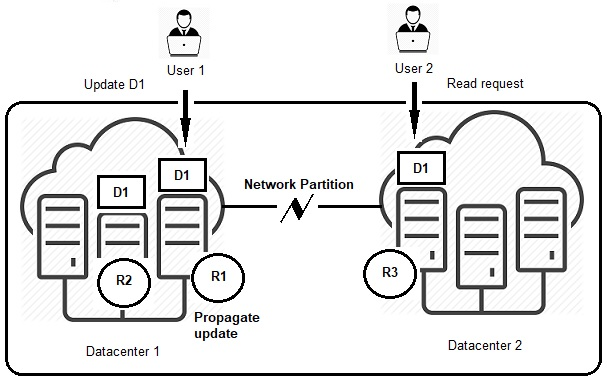
\includegraphics[width=0.47\textwidth]{fig1.jpg}
\caption{Consistency versus Availability in Replicated Systems.}
\label{fig:figure1}
\end{figure}

\vspace{1mm}
The realization of the trade-offs caused by the CAP theorem led to the proliferation of not-ACID models for building cloud-based applications, {\al {\it i.e.,}} systems that are {\al {\it Basically Available}}, rely on the maintenance of a {\al {\it Soft state} that can} be rebuilt in case of failures and are only {\al {\it Eventually consistent}} to be able to survive network partitions. %That 
{\al Such a} model became know as BASE~\cite{sosp1997base} and may offer different consistency models, which are discussed next. 
%in Section~\ref{sec:consistencymodels}.
\\
%\vspace{1mm}



